	\documentclass[11pt]{article}
	
	\title{Homework 1 - DM CS6220}
	\author{Nakul Camasamudram}
	\usepackage{amsmath,amsfonts,amsthm} % Math packages
	\usepackage{mathtools}
	\usepackage{adjustbox}
	%----------------------------------------------------------------------------------------
	%	TITLE SECTION
	%----------------------------------------------------------------------------------------
	
	\newcommand{\horrule}[1]{\rule{\linewidth}{#1}} 
	
	\title{	
	\normalfont \normalsize 
	\textsc{Northeastern University, Data Mining Techniques - CS6220 Fall 2017} \\
	 % Your university, school and/or department name(s)
	\horrule{0.5pt} \\[0.4cm] % Thin top horizontal rule
	\huge Solutions to Homework 2, Part 2 \\ % The assignment title
	\horrule{2pt} \\[0.5cm] % Thick bottom horizontal rule
	}
	\author{Nakul Camasamudram} % Your name
	\date{\normalsize\today} % Today's date or a custom date
	\begin{document}
	
	\maketitle % Print the title
	\newpage
	
	%----------------------------------------------------------------------------------------
	%	PROBLEM 1
	%----------------------------------------------------------------------------------------
	
	\section*{1. K-Means}

	\textbf{Solution:}\\
    
    \begin{itemize}
    	\item \textbf{Iteration 1:} \\
    	The initial centroids are $C_1$ = (2, 10) $C_2$ = (1, 2) $C_3$ = (5, 8). Let D($C_i$) represent the \textbf{euclidean} distance between the respective point and the $i^{th}$ centroid.
    	
		\underline{The $E$-step:} \\
    		\begin{center}
    			\begin{adjustbox}{max width=\textwidth}
				\begin{tabular}{ | c | l | l | l | l |}
	  	 		\hline
    				\textbf{Data Point} & \textbf{D($C_1$)} & \textbf{D($C_2$)} & \textbf{D($C_3$)} & \textbf{Optimal centroid} \\ 
    			\hline
    				(4,9) & 2.23606797749979 & 7.615773105863909 & \textbf{1.4142135623730951} & $C_3$ \\ 
    			\hline
    				(2,10) & \textbf{0.0} & 8.06225774829855 & 3.605551275463989 & $C_1$ \\ 
    			\hline
					(1,2) & 8.06225774829855 & \textbf{0.0} & 7.211102550927978 & $C_2$ \\ 
    			\hline   
    				(2,5) & 5.0 & \textbf{3.1622776601683795} & 4.242640687119285 & $C_2$ \\ 
    			\hline
	    			(6,4) & 7.211102550927978 & 5.385164807134504 & \textbf{4.123105625617661} & $C_3$ \\ 
    			\hline
    				(8,4) & 8.48528137423857 & 7.280109889280518 & \textbf{5.0} & $C_3$ \\ 
    			\hline
    				(7, 5) & 7.0710678118654755 & 6.708203932499369 & \textbf{3.605551275463989} & $C_3$ \\ 
    			\hline 	
    				(5, 8) & 3.605551275463989 & 7.211102550927978 & \textbf{0.0} & $C_3$ \\ 
    			\hline 					
    			\end{tabular}
    			\end{adjustbox}
		\end{center}
		
		\underline{The $M$-step:} \\
		$C_1$ = mean[(2, 10)] = (2.0, 10.0) \\
		$C_2$ = mean[(1, 2), (2, 5)] = (1.5, 3.5) \\
		$C_3$ = mean[(4, 9), (6, 4), (8, 4), (7, 5), (5, 8)] = (6.0, 6.0) \\
		
		\begin{center}
			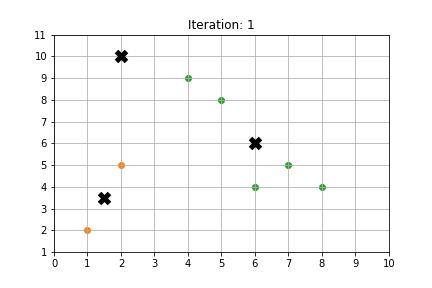
\includegraphics[scale=0.7]{kmeans_graphs/iteration_1.png}
		\end{center}

    	\item \textbf{Iteration 2:} \\
		\begin{center}
			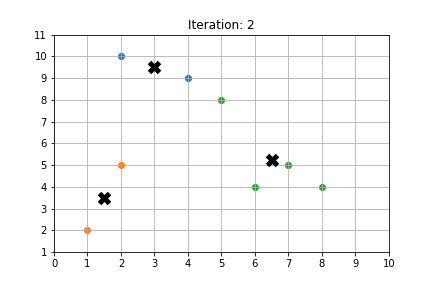
\includegraphics[scale=0.7]{kmeans_graphs/iteration_2.png}
		\end{center}
		
		\item \textbf{Iteration 3:} \\
		\begin{center}
			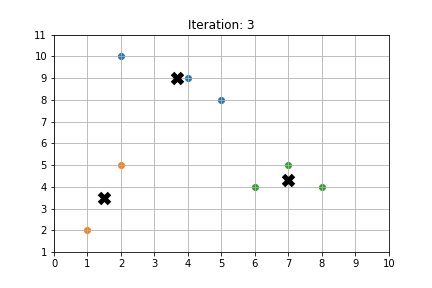
\includegraphics[scale=0.7]{kmeans_graphs/iteration_3.png}
		\end{center}
		
		\item \textbf{Iteration 4:} \\
		\begin{center}
			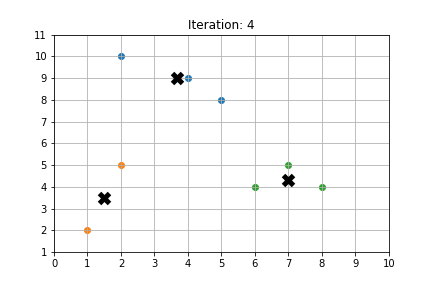
\includegraphics[scale=0.7]{kmeans_graphs/iteration_4.png}
		\end{center}
    \end{itemize}
	\newpage
	
	%----------------------------------------------------------------------------------------
	%	PROBLEM 2
	%----------------------------------------------------------------------------------------
	\section*{2. Agglomerative Hierarchical}

	\textbf{Solution:}\\
	\newpage
	
	
	%----------------------------------------------------------------------------------------
	%	PROBLEM 3
	%----------------------------------------------------------------------------------------
	\section*{3. DBSCAN}

	\textbf{Solution:}\\
	\newpage
\end{document}




























